\documentclass[apj]{emulateapj}

\usepackage{biblatex}
\addbibresource{biblio.bib}

\usepackage{graphicx}
\usepackage{hyperref}
\usepackage{epsfig}
\usepackage{amssymb, amsmath}
\usepackage{array}
\usepackage{threeparttable}


\singlespace

%definitions
\newcommand{\Msol}{${\rm M_{\sun}}$}


%% Editing markup...
\usepackage{color}


%%%%%%%%%%%%%%%%%%%%%%%%%%%%%%%%%%%%%%%%%%%%%%%%%%%%%%%%%%%%%%%%%%%%%%%%%%%
% WARNING: This LaTeX block was generated automatically by authors.py
% Do not change by hand: your changes will be lost.

%%%%%%%%%%%%%%%%%%%%%%%%%%%%%%%%%%%%%%%%%%%%%%%%%%%%%%%%%%%%%%%%%%%%%%%%%%%


% --------------------- Ancillary information ---------------------
\shortauthors{Horlaville}
\shorttitle{Exploring Line Intensity Cube Predictions with \MakeLowercase{\texttt{limlam$\_$mocker}}}
\slugcomment{Draft: \today}


\begin{document}

\title{Exploring Line Intensity Cube Predictions with \MakeLowercase{\texttt{limlam$\_$mocker}}}
%Investigating Dark Matter Halos Through Line Intensity Fluctuations
 %% ---------
 
\author{Patrick Horlaville\altaffilmark{1}^{,}\altaffilmark{2}}
\altaffiltext{1}{CITA, University of Toronto}
 \altaffiltext{2}{McGill University}
\keywords{cosmology: galaxy --- dark matter --- CO line intensity}



\section{Introduction}
\label{sec:intro}
\subsection{Background}
The study of high redshift galaxies is increasingly important in the context of our understanding of galaxy formation and cosmology. While modern surveys still struggle to efficiently probe those populations, simulation techniques such as intensity mapping have proven to be able to infer the properties of those dear high redshift galaxies, \textit{e.g}. intensity mapping of carbon monoxide and its ground-state transition (Li et al., 2016) \cite{Li_2016}.

Intensity mapping (IM), or line intensity mapping (LIM), is a technique that consists of probing the 3D sky (RA, Dec \& $\nu_{obs}$) at low angular resolution of specific molecular lines (Karkare, $n.d.$ \cite{Karkare}). The strength of this analysis resides in 1) its potential to probe large cosmological volume quickly and 2) its ability to probe galaxies invisible to standard galaxy surveys. 

\subsection{Related to the Project}

The goal of this project is to analyze how predicted galaxies' properties as found by Li et al. (2016) \cite{Li_2016} compare to those of a Python program named \texttt{limlam$\_$mocker}. The two aim to perform a line intensity analysis using CO emission over dark matter halos, which allows to compute their CO brightness temperature. However, two main differences are to be considered. First, the average redshift of the probed halos are not the same for the two analyses. The population used by Li et al. (2016) \cite{Li_2016} has $z$ $\sim$ [2.4, 2.8]. For the \texttt{limlam}\_\texttt{mocker} comparison, refer to Fig. \ref{fig:zdist}. Second, the method used to identify those halos are not the same. This will be elaborated upon later.

Both analyses consider a minimum cutoff for halos' mass. Indeed, low-mass halos are not expected to be CO-bright as they are expected to be poor of systems rich in dust or metal (Li et al., 2016) \cite{Li_2016}. Then, how does the CO brightness temperature depend on the chosen mass cutoff? The final objective of this project would be to use \texttt{limlam$\_$mocker} to determine this relationship and compare it to the result of Li et al. (2016). 


\section{Process}
\label{sec:process}
\subsection{Getting Started}
To first get started with the \texttt{limlam$\_$mocker} program, I cloned it to my home repository in my CITA environment. From there, I looked into some of its objects. The first one is a lightcone simulation output within the \texttt{catalogues} directory. It notably contains the virial mass (in solar masses $\rm{M_\odot}$) and the redshift $z$ of every halo. Fig. \ref{fig:massdist} and \ref{fig:zdist} display the \texttt{Log}(mass) and redshift distribution of those halos present in our catalogue.

\begin{figure}[h!]
  \centering
  \begin{subfigure}
    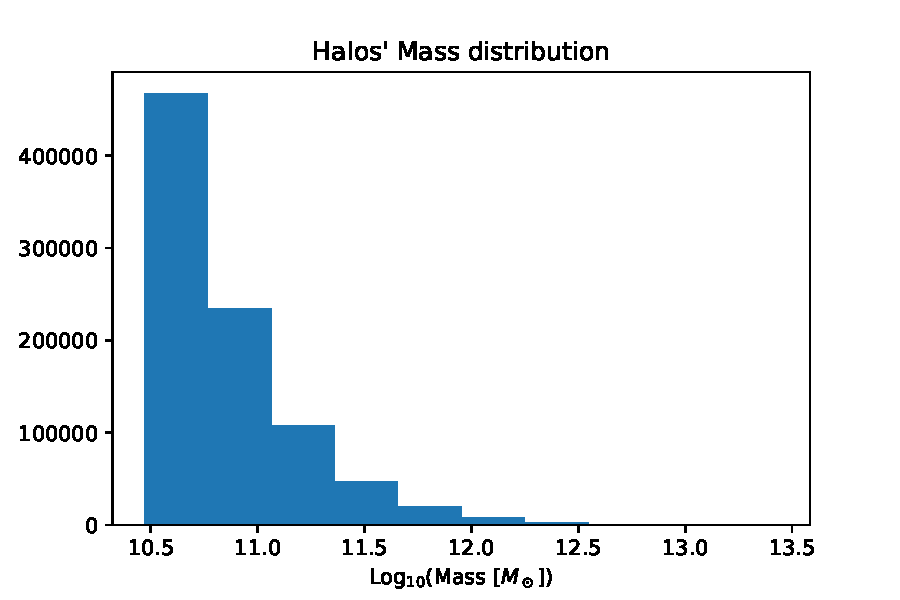
\includegraphics[width=\linewidth]{mass_distribution.pdf}
  \caption{Here shown is the distribution of halos' \texttt{Log}(masses) from the catalog used in our \texttt{limlam}\_\texttt{mocker} analysis. As indicated by the exponential $x$-scale, we have M $\sim$ [$10^{10}$, $10^{13}$] $\rm{M}_\odot$ for our catalog.}
  \label{fig:massdist}
  \end{subfigure}
  \begin{subfigure}
    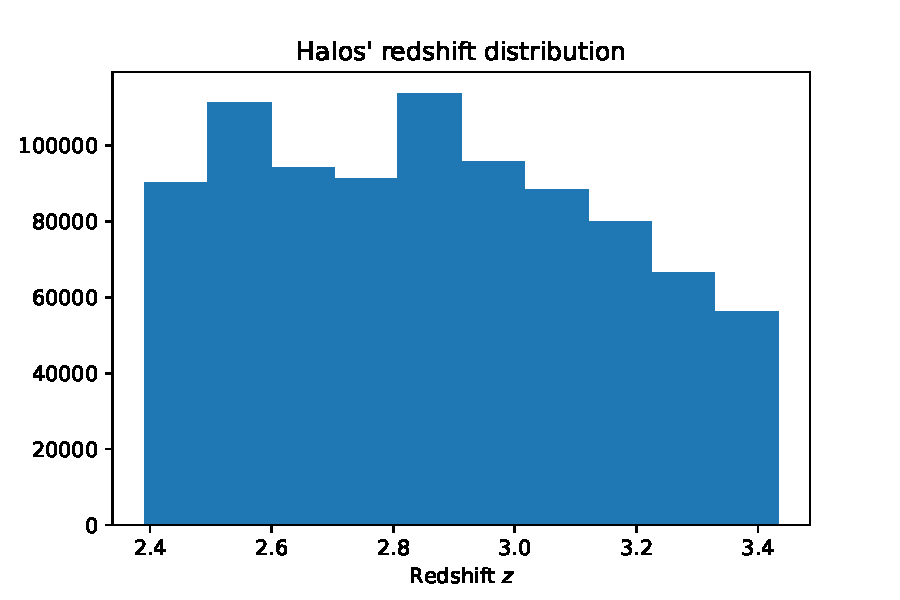
\includegraphics[width=\linewidth]{redshift_distribution.pdf}
  \caption{Here shown is the distribution of halos' redshifts from the catalog used in our \texttt{limlam}\_\texttt{mocker} analysis. This population of halos differs to the one of Li et al. (2016) as a significant part of it has $z$ \in [2.8, 3.4].}
  \label{fig:zdist}
  \end{subfigure}
\end{figure}

\subsection{Tweaking the Code}
Since the inception of \texttt{limlam}\_\texttt{mocker}, \texttt{numpy} and possibly other packages upon which the program depends upon have changed so that running the code as it is yields an error. This error was solved by adding the argument \texttt{allow}\_\texttt{pickle = True} while loading the halo catalogue in the file \texttt{load}\_\texttt{halos.py}. 

\pagebreak

\subsection{Running the Code}
The file performing the line intensity mapping, \texttt{lim}\_\texttt{mocker.py}, can now be ran. Now that this is solved, we can investigate how the program works in its great lines.

First, a mock map is being generated out of parameters specified in the file \texttt{params.py}. Then, \texttt{load}\_\texttt{peakpatch}\_\texttt{catalogue} allows to load the halos from the catalogue. After being loaded, the halos undergo the minimum mass cutoff with \texttt{cull}\_\texttt{peakpatch}\_\texttt{catalogue}. From there, multiple routes are possible to retrieve the CO brightness temperature of our halos. Here we follow the procedure prescribed by Li et al., 2016 \cite{Li_2016}, which is the default method in the \texttt{limlam}\_\texttt{mocker} package. The halo mass densities can be translated to stellar mass functions, which are then related to star formation rates (SFR). Given SFRs are not directly observable, they can be inferred from spectral tracers such as the total infrared luminosity $L_{\rm{IR}}$ as given by Equation \ref{eq:SFR}:


\begin{equation}
    \rm{SFR} = \delta_{\rm{MF}} \times 10^{-10}  L_{\rm{IR}}.
    \label{eq:SFR}
\end{equation}

The infrared luminosity can then be converted to CO luminosity as given by Equation \ref{eq:LIR}, where the relationship between the two is assumed to be a power law with parameters $\alpha$ and $\beta$:

\begin{equation}
    \rm{log} \hspace{1mm} L_{\rm{IR}} = \alpha \hspace{1mm} \rm{log} L_{CO}' + \beta,
    \label{eq:LIR}
\end{equation}

where the units of $\rm{L_{IR}}$ are $\rm{L_\odot}$ and those of $\rm{L_{CO}'}$ are K km $\rm{s^{-1}}$ $\rm{pc^{-2}}$. Li et al., 2016 \cite{Li_2016} use values of $\alpha$ = 1.37 and $\beta$ = -1.74 from a census of high-redshift galaxies.

$\rm{L_{CO}'}$ can be converted into $\rm{L_{CO}}$ (with units of $\rm{L_\odot}$) as per Equation \ref{eq:LCOPtoLCO}:

\begin{equation}
    \rm{L_{CO}} = \textit{A} \times \rm{L_\odot} (\frac{\rm{\nu_{CO, rest}}}{115.27 GHz})^3 (\frac{\rm{L_{CO}'}}{K \hspace{1mm} km \hspace{1mm} s^{-1} \hspace{1mm} pc^{-2}}),
    \label{eq:LCOPtoLCO}
\end{equation}

where $A$ is a fudge factor of $4.9 \times 10^{-5}$ and $\rm{\nu_{CO, rest}}$ is the rest-frame frequency of the CO transition (115.27GHz). The brightness temperature, finally, can be found through the Rayleigh-Jeans relation as shown in Equation \ref{eq:Ray}:

\begin{equation}
    T = \frac{c^2 I_{\nu, obs}}{2k_b \nu_{obs}^2}
    \label{eq:Ray}
\end{equation}

where $k_b$ is the Boltzmann constant and $I_{\nu, obs}$ = $\frac{L_{CO}}{4\pi D_L^2 \delta_{\nu}}$, inside which $D_L$ is the luminosity distant to the source, $\delta_{\nu}$ is the width of the spectral resolution element, a parameter determined by the prospective resolution of future instruments that will carry on those observations.

One of the outputs of the program, an \texttt{.npz} file, contains the sought-after CO brightness temperature for every point in our grid.

\subsection{Loading Results}
Each run of \texttt{limlam}\_\texttt{mocker.py} corresponds to finding the CO brightness temperature across all of our map for one specified threshold of minimum mass. If we run it three times with min. mass = $3 \times 10^{10}, 10^{11} \hspace{1mm} \rm{and} \hspace{1mm} 10^{12} \rm{M_\odot}$, we can take the average over the cube of the CO brightness temperature at each time and compare this preliminary result with the results found by Li et al. (2016) \cite{Li_2016} between the minimum mass threshold chosen and the resulting average CO brightness temperature. The results are shown in Fig. \ref{fig:tco_coarse}


\begin{figure}[h!]
  \centering
    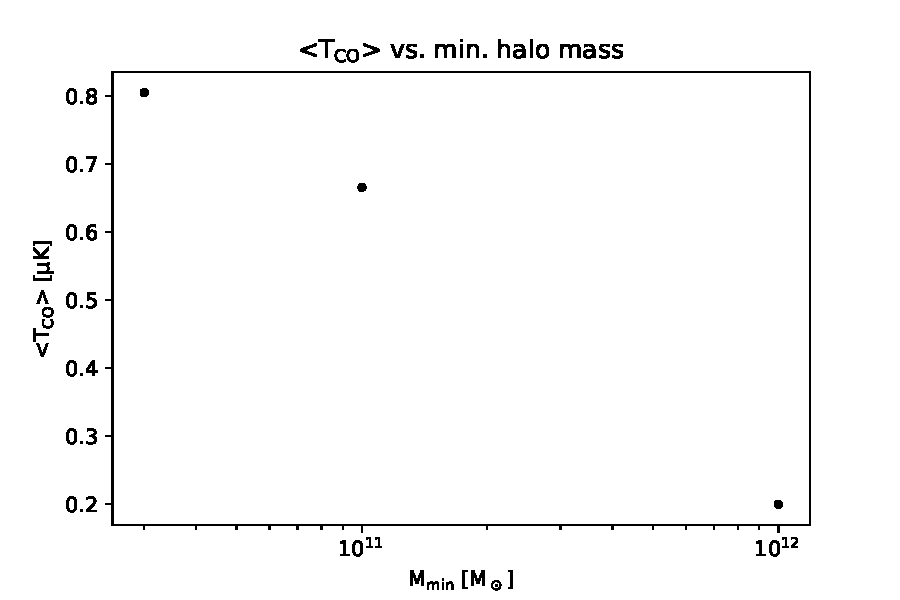
\includegraphics[width=\linewidth]{tco_coarse.pdf}
  \caption{Here shown are the results from 3 runs of the \texttt{limlam}\_\texttt{mocker} analysis using different minimum halo mass thresholds. The values found are compared with their equivalent from Li et al. (2016) \cite{Li_2016} in Table \ref{tab:val}. }
  \label{fig:tco_coarse}
  \end{figure}
  
  
  
  

\begin{table}[h!]
\begin{center}
\begin{threeparttable}
\caption{Comparison of results between Li et al. (2016) \cite{Li_2016} and \texttt{limlam}\_\texttt{mocker}.}
\begin{tabular}{|l|c|c|}
\hline 
   & Min. Mass [$\rm{M_\odot}$] & $<T_{CO}> [\mu K]$ \\
 \hline  
\texttt{limlam}\_\texttt{mocker} & $3 \times 10^{10}$ & 0.80 \\
Li et al. (2016) \cite{Li_2016} & $1 \times 10^{10}$ & 0.92 \\
\hline
\texttt{limlam}\_\texttt{mocker} & $1 \times 10^{11}$ & 0.67 \\
Li et al. (2016) \cite{Li_2016} & $1 \times 10^{11}$ & 0.67 \\
\hline 
\texttt{limlam}\_\texttt{mocker} & $1 \times 10^{12}$ & 0.20 \\
Li et al. (2016) \cite{Li_2016} & $1 \times 10^{12}$ & 0.26 \\
\hline 
\end{tabular} 
\vskip 2mm
\begin{tablenotes} \item  
\begin{center}
\begin{flushleft}
Notice that both methods seem to give results of the same order. This comparison is investigated further in the next section.
\end{flushleft}
\end{center}
\end{tablenotes}
\label{tab:vitalStats_kappa}
\end{threeparttable}
\end{center}
\label{tab:val}
\end{table}

\subsection{Iterating Over a Lot of Minimum Masses}
Rather than being stuck with three data points, we would like to have a continuous-like array of minimum masses and corresponding average CO brightness temperature values to better establish the relationship between those two quantities. To do so, I modified the scripts from the \texttt{limlam}\_\texttt{mocker} repo so as to integrate notably \texttt{N}, the number of desired iterations as well as \texttt{ubound} and \texttt{lbound}, the upper and lower bound on the log space of values over which the iterations are being performed. A few functions have to be adapted here and there, but it's mainly a matter of integrating a \texttt{for} loop over all the process. The resulting relationship is shown in Fig. \ref{fig:tco_full}. The equivalent result from Li et al. (2016) \cite{Li_2016} is shown in Fig. \ref{fig:tco_li}. 

\pagebreak


\begin{figure}[h!]
    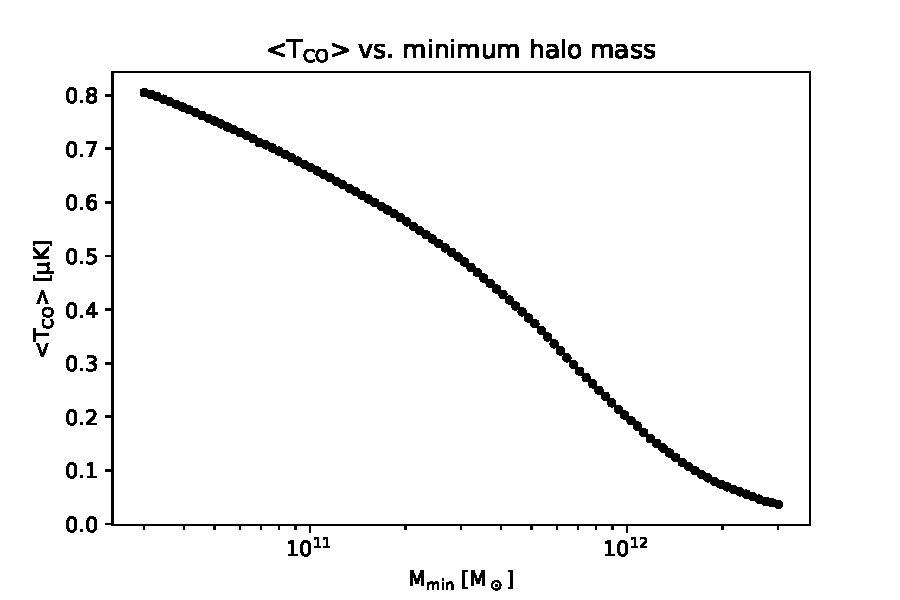
\includegraphics[width=\linewidth]{tco_full.pdf}
  \caption{Here shown are the results from 100 runs of the new \texttt{limlam}\_\texttt{mocker} program, namely \texttt{new}\_\texttt{llm}. The values chosen for the iteration were \texttt{lbound} $ = 3 \times 10^{10}$, \texttt{ubound} $ = 3 \times 10^{12}$ [in $\rm{M\odot}$] and $N$ = 100. We can compare this graph to Figure 11 from Li et al. (2016) \cite{Li_2016}, as shown in Fig. \ref{fig:tco_li}. }
  \label{fig:tco_full}
\end{figure}
  
\begin{figure}[h!]
  \centering
  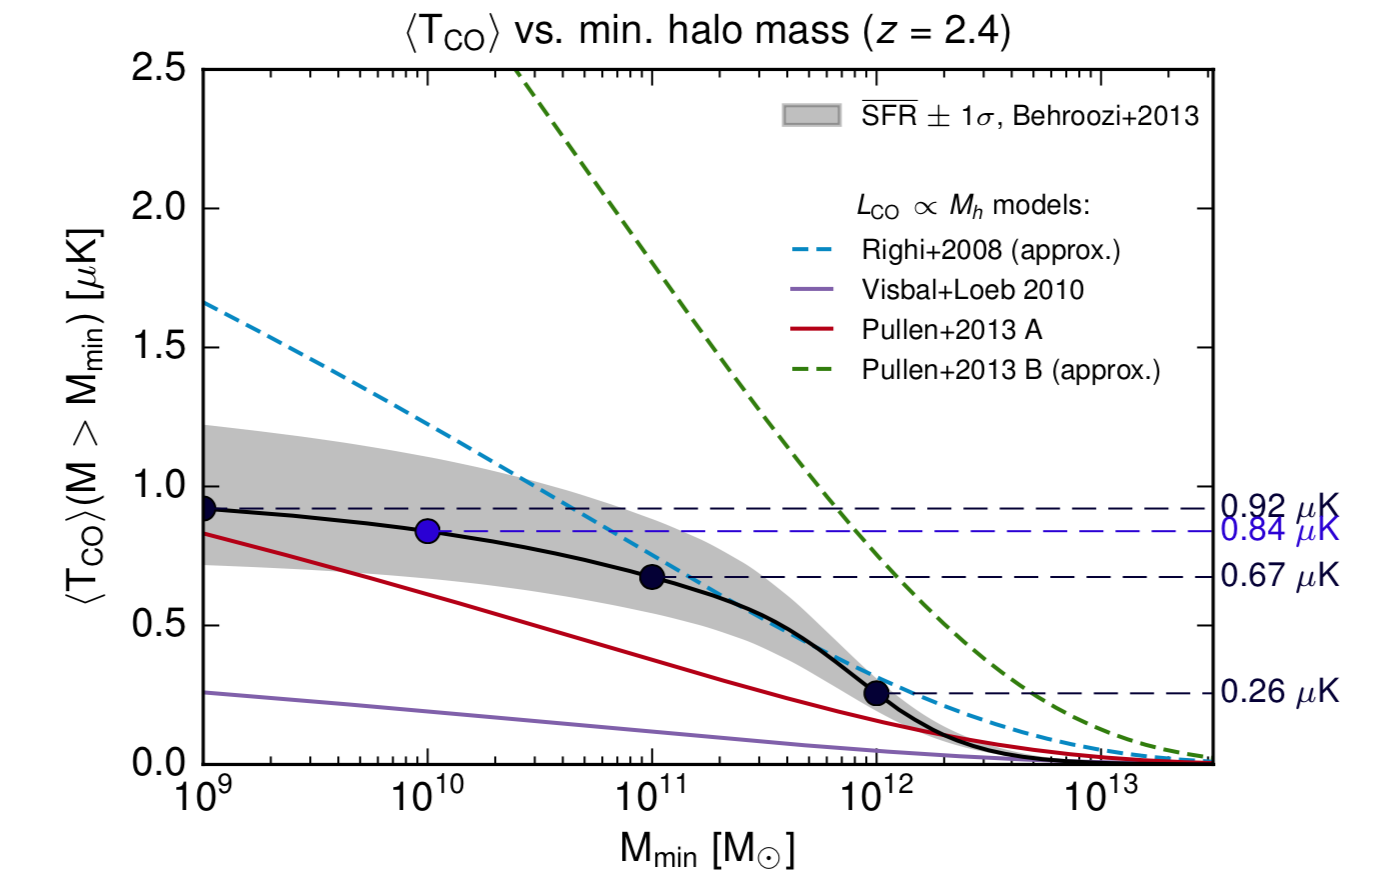
\includegraphics[width=\linewidth]{li_fig11.png}
  \caption{Here shown is Figure 11 of Li et al. (2016) \cite{Li_2016}, displaying the relationship between the chosen minimum halo mass and the corresponding average CO brightness temperature [in black].}
  \label{fig:tco_li}
\end{figure}

\section{Discussion \& Conclusion}
Fig. \ref{fig:tco_full} and Fig. \ref{fig:tco_li} show a qualitative match between the \texttt{limlam}\_\texttt{mocker} and the Li et al. (2016) \cite{Li_2016} relationship between $\rm{M_{min}}$ and $<T_{CO}>$


This is already remarkable given the different methods used. Li et al. (2016) \cite{Li_2016} had recourse to a cosmological $N$-body dark matter simulation to retrieve the dark matter halos, which is computationally very expensive compared to the method used by \texttt{limlam}\_\texttt{mocker}: the Peak Patch method. The mass-Peak Patch method allows to look into very large volumes of halo catalogues without having to go into the numerical dread of $N$-body simulations. Despite being a more approximate method, the mass-Peak Patch method has proven to be efficient for creating large volumes of halo catalogues (Stein et al., 2018 \cite{Stein_2018}). Here, it seems to have predicted the relationship between halo minimum mass cutoff and average CO brightness temperature just as an $N$-body simulation would have.

The functionality of the mass-Peak Patch method promises to be of help in the simulation of large cosmological dark matter halo populations. I hope I can get to make interesting use of this tool in the prospect of my research work this summer, notably in other contexts like C II line intensity mapping.

\printbibliography


\end{document}
